\documentclass[A5,11pt]{article}
\usepackage[utf8]{inputenc}
\usepackage[spanish]{babel}
\usepackage[rmargin=2.5cm, lmargin=3cm, tmargin= 3cm, bmargin=3cm]{geometry}
\usepackage[svgnames,x11names,dvipsnames]{xcolor} 
\usepackage{graphics}
\usepackage[rightcaption]{sidecap}
\usepackage{caption}

%---------COLORES--------------------
\usepackage{graphicx}
\definecolor{azulito}{RGB}{40, 190, 188}
\definecolor{r0jo}{RGB}{190, 40, 74}
\definecolor{v3rd3}{RGB}{83, 190, 40}
\definecolor{amarill0}{RGB}{190, 183, 40 }

\pagecolor{black} %color a la hoja
\color{white} %color de letra

%http://latexcolor.com/ 
%-----------CABECERA-----------------
\usepackage{fancyhdr}%paqueteria para modificar encabezados
\pagestyle{headings} %cabecera 
\pagestyle{fancy} %pone la paqueteria
    \rfoot{página \thepage}
    \cfoot{}
    \lfoot{Méndez González Romina Estephania}
%---------------------------------



\begin{document}

\begin{center}
    \textbf{\Large{\emph{Les presento a la serie que me hizo llorar un montón, solo porque soy romántica y me llegó mucho en el corazón $<$/3}}}
\end{center}

\section{\emph{Descripción fachera facherita}}
    \subsection{Reseña cool}
        La serie ``The End of the F***ing World''fue transmitida por primera vez en la plataforma Netflix en el año 2017. La serie cuenta con dos temporadas, ambas con 8 episodios. Explicare solo la primera temporada porque fue la que más me gustó. En general, la primera temporada narra la vida de dos adolescentes: Alyssa y James, los cuales, van en la misma escuela y por azares del destino se conocen un día en el almuerzo. Es importante puntualizar que Alyssa y James son dos personas que desde el inicio de sus vidas presenciaron experiencias muy traumáticas y tristes, por tanto ambos perseguían objetivos particulares; en este caso, Alyssa quería comenzar una nueva vida, alejada de su familia disfuncional y James quería confirmar si era un psicópata. Así pues, Alyssa y James se vuelven novios y un día deciden tener una cita en la casa de James, pero él planeaba matarla; sin embargo, en un arranque de emociones deciden escaparse en el carro del papá de James. Conduciendo sin rumbo, James choca el auto y deciden entrar a una casa en la que aparentemente nadie vive. Alissa y James beben alcohol, ponen música, bailan, comen y disfrutan el momento, pero cuando van a dormir llega el dueño de la casa. Tal individuo intenta abusar sexualmente de Alyssa, así que James la defiende y mata al individuo. Posteriormente, James se da cuenta que no era un psicópata y siente culpa por matar a alguien. Tras lo ocurrido, la policía comienza a buscar a Alissa y James. Con esto, Alyssa (acompañada con James) decide irse con su padre; sin embargo, Alyssa no confía en James por lo ocurrido así que se escapa de él. James se pone muy triste por haber intentado matar a Alyssa, a demás, se da cuenta que la empieza a amar. A los pocos días, ambos se encuentran en la calle, sin rumbo y muy tristes. Ambos, con el corazón, el alma y la mente rota deciden juntarse e ir a un lugar ``seguro'': con el papá de Alyssa. Cuando llegan con él, Allysa se siente segura, pero tiempo después, su papá los entrega a la policía a cambio de recibir dinero. Antes de que la policía llegue por Alissa y James, ellos se dan cuenta y deciden huir, pero es muy tarde ya que le disparan el la pierna a James y con la culpa que siente por haber matado, decide entregarse a la policía. Así es como termina la primera temporada.
        
    \subsection{Elenco}
        \begin{enumerate}
            \item Alex Lawther: Personaje principal
            \item Jessica Barden: Personaje principal
            \item Gemma Whelan: Personaje principal
            \item Wunmi Mosaku: Personaje principal
            \item Steve Oram: Personaje secundario
            \item Christine Bottomley: Personaje secundario
            \item Navin Chowdhry: Personaje secundario
            \item Barry Ward: Personaje secundario
            \item Jonathan Entwistle: Creador y director
            \item Ed Macdonald: Productor
            \item Kate Ogborn: Productor
        \end{enumerate}
        
    \subsection{Personajes}
        \begin{itemize}
            \item [$\heartsuit$] \fcolorbox{blue}{r0jo}{James: Chico de 17 años que creyó ser un psicópata. Es el amorio de Alyssa.  }
            \item [$\heartsuit$] \fcolorbox{blue}{azulito}{Alyssa: Chica de 17 años, incomprendida, odia a todo el mundo y es el amorio de James. }
            \item [$\heartsuit$] \fcolorbox{blue}{v3rd3}{Eunice: Policía a cargo de la investigación por el asesinato. }
            \item [$\heartsuit$] \fcolorbox{blue}{amarill0}{Teri: Compañera de investigación de Eunice (está enamorada de Eunice). }
            \item [$\heartsuit$] Gwen: Madre de Alyssa. Tiene problemas de apego y no sabe tomar decisiones.
            \item [$\heartsuit$] Phil: Padre biológico de Alyssa. Es un dealer, no es responsable de sus hijos y no los quiere.
            \item [$\heartsuit$] Tony: Padrastro de Alyssa. Tiene dos hijos con Gwen pero desprecia y maltrata psicológicamente a Alyssa. 
        \end{itemize}
        
    \subsection{Imagen de esta bella serie }
        \begin{figure}[h]\raggedleft
            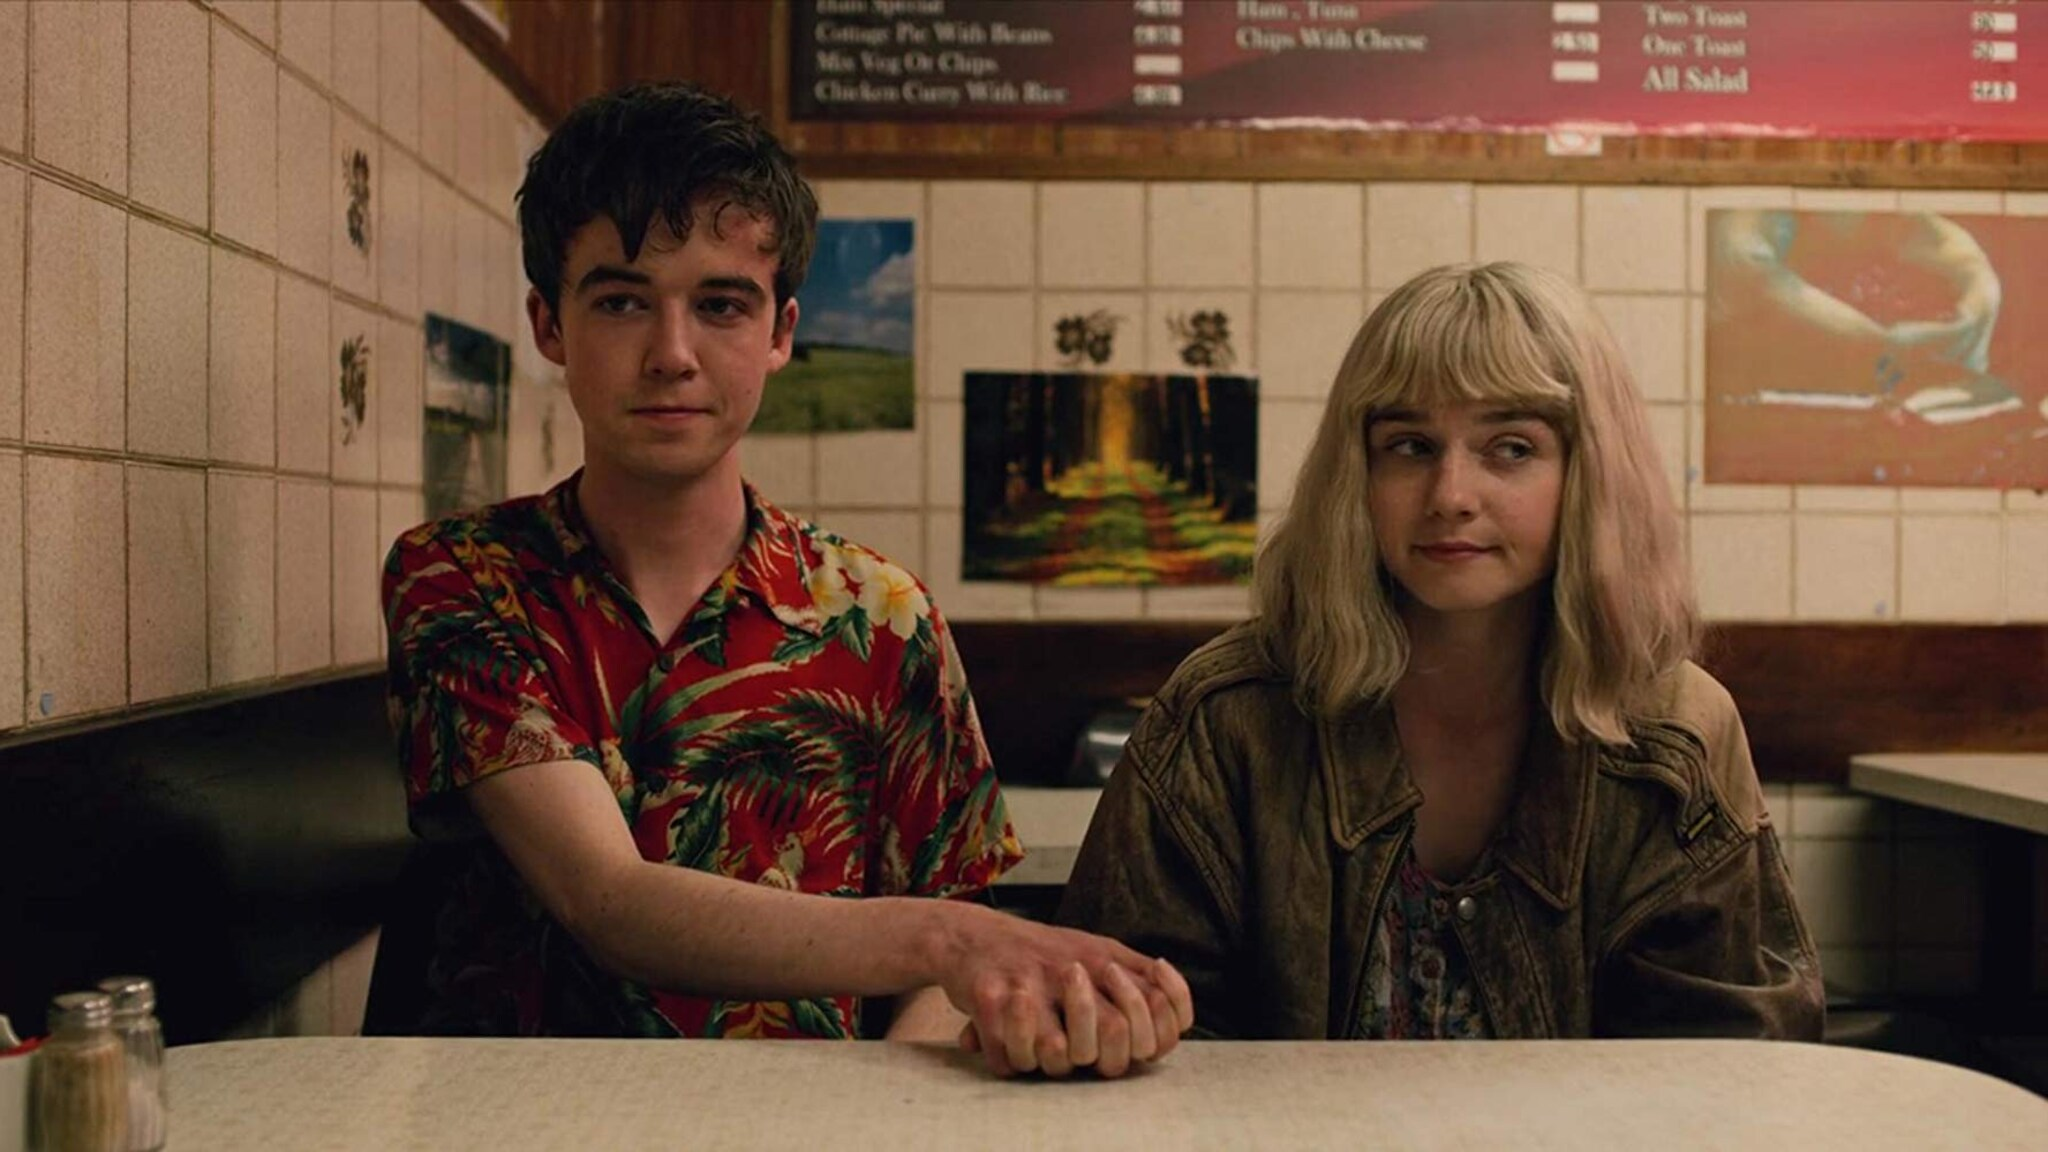
\includegraphics[angle=15, scale=0.12]{Imagenes/The end.jpg}
            \caption*{La pareja más trágica que puede existir en toda la vida}
        \end{figure}
    
    %Aquí está la frase del margen uwu   
    \hspace{-3cm}{\emph{She made me }}\\ .
    \hspace{-2.7cm}{\emph{feel things...}}\\
    
    
    
         
\section{\emph{¿Por qué esta serie?}}
    \textcolor{Tan}{Decidí esta serie porque hace poco estaba pensando en verla nuevamente; a demás, esta serie me genera un sentimiento de \emph{nostalgia inexplicable}.} 
    \textcolor{BrickRed}{Cuando vi esta serie, yo iba en la secundaria y había pasado por una relación demasiado inestable... así que el contenido de esta serie me ayudó a reflexionar y darme cuenta que muchas actitudes dentro de una relación no son sanas. También, entendí como es que se puede ver la dependencia emocional y porqué puede surgir. }\\
    \textcolor{SeaGreen}{Finalmente, el tema por el que escogí esta serie (y creo que es el más importante) es porque mi personalidad es afín a la de la protagonista, pues le irritan muchas personas de su colegio, no le gustan los bebes pero le gusta que sus cabezas huelan a vainilla, \emph{ignora a su crush aunque lo ame} y a demás, muchas vivencias que he tenido, ella también las pasó.} Creo que escogí esta serie por muchas razones, ya que trata muchos temas que tienen un trasfondo muy profundo y puede impactar dependiendo la vida de cada persona.  
    
    \subsection{Personaje con el que me casaría porque somos almas gemelas}
        \begin{SCfigure}[1][h]
            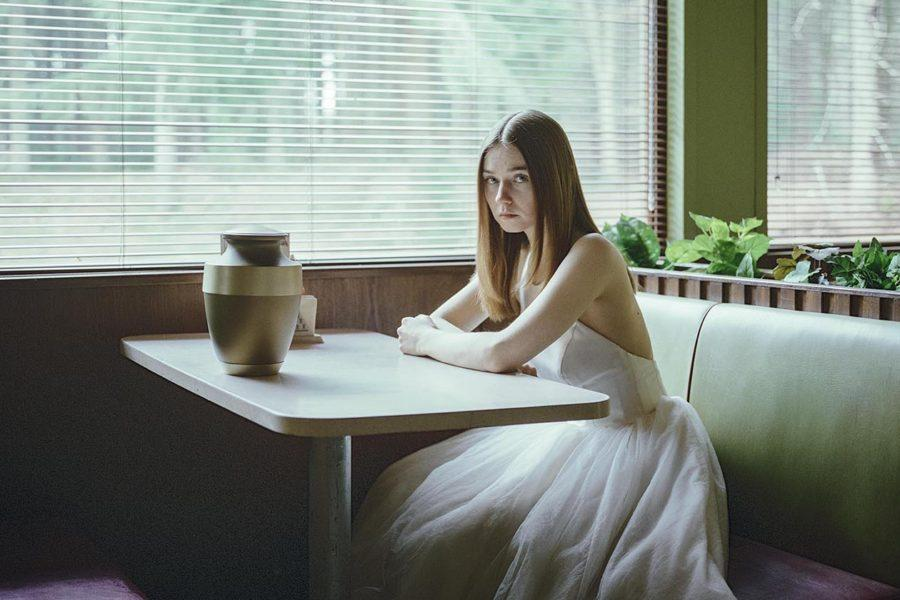
\includegraphics[angle= -18, scale=0.19]{Imagenes/Alyssa.jpg}
            \caption{ Alyssa: Protagonista que desempeña el papel de          una adolescente emocional e incomprendida y que          tiene sentimientos por James.}
        \end{SCfigure}
        
        
    \subsection{Personaje que me cae mal porque se parece a mi papá}
        \begin{SCfigure}[1][h]
            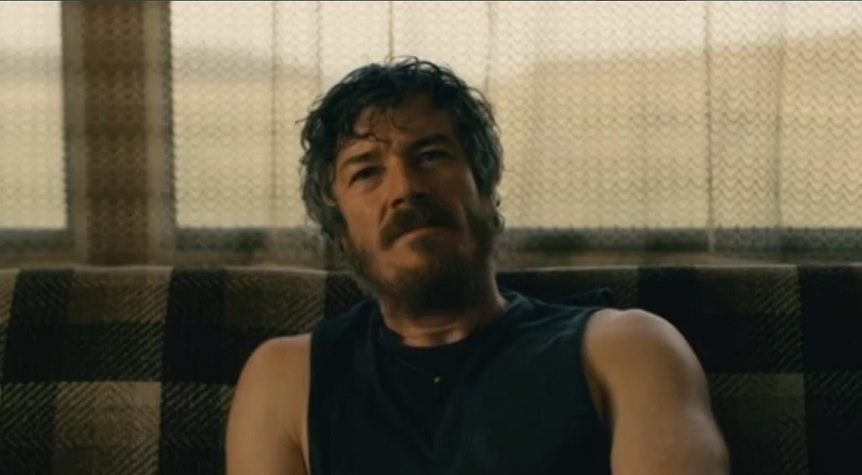
\includegraphics[angle= 8, scale=0.37]{Imagenes/Phil.jpg}
            \caption{Phil: Papá irresponsable que tiene muchos hijos         y no se hace cargo de ninguno de ellos, es              alcohólico y fumador.}
        \end{SCfigure}
        
\end{document}
